\documentclass{standalone}

\usepackage{tikz}
\usetikzlibrary{automata,positioning}
\begin{document}
% \begin{tikzpicture}[shorten >=1pt,node distance=2cm,on grid,auto] 
%    \node[state,initial] (q_0)   {$q_0$}; 
%    \node[state] (q_1) [below=of q_0] {$q_1$}; 
%    \node[state] (q_2) [below left=of q_1]  {$q_2$}; 
%    \node[state] (q_3) [below right=of q_2] {$q_3$}; 
%    \node[state,accepting](q_4) [below right=of q_1] {$q_4$};
%     \path[->] 
%     (q_0) edge node {True}  (q_1)
%     (q_1) edge [loop right] node {$\neg$P} ()
%           edge[bend left]  node {P} (q_2)
%     (q_2) edge  node [swap] {P} (q_3)
%           edge[bend left]  node {$\neg$P} (q_1)
%     (q_3) edge  node [swap] {D} (q_4) 
%           edge [loop right] node {$\neg$D} ();
% \end{tikzpicture}


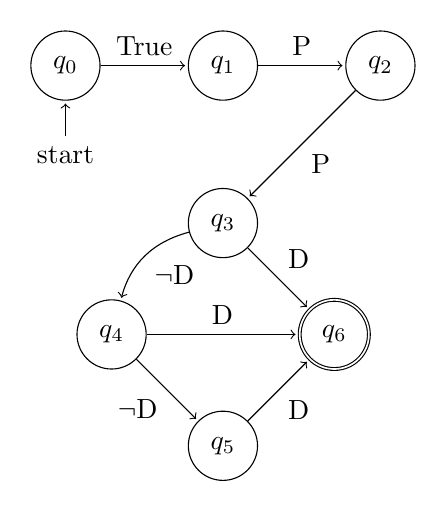
\begin{tikzpicture}[shorten >=1pt,node distance=2cm,on grid,auto] 
   \node[state,initial below] (q_0)   {$q_0$}; 
   \node[state] (q_1) [right=of q_0] {$q_1$}; 
   \node[state] (q_2) [right=of q_1] {$q_2$}; 
   \node[state] (q_3) [below=of q_1] {$q_3$}; 
   \node[state] (q_4) [below left=of q_3]  {$q_4$}; 
   \node[state] (q_5) [below right=of q_4] {$q_5$}; 
   \node[state,accepting](q_6) [below right=of q_3] {$q_6$};
    \path[->] 
    (q_0) edge node {True}  (q_1)
    (q_1) edge node {P}  (q_2)
    (q_2) edge node {P}  (q_3)
    (q_3) edge[bend right]  node {$\neg$D} (q_4)
          edge node {D} (q_6)
    (q_4) edge  node [swap] {$\neg$D} (q_5)
          edge node {D} (q_6)
    (q_5) edge  node [swap] {D} (q_6);
\end{tikzpicture}



%  mdp
% \begin{tikzpicture}[shorten >=1pt,node distance=2cm,on grid,auto] 
%    % Define nodes
%   \node[state,initial] (x_0) {$s_0$}
%   node[below=0.5cm] {\{P\}};
%   \node[state] (x_1) [right of=x_0] {$s_1$}
%     node[below=0.8cm of x_1] {\{D\}}; 
  
%   % Edges
%   \path[->] 
%     (x_0) edge[loop above] node {$a_0$, 0.2} (x_0)
%     (x_0) edge[bend left] node {$a_0$, 0.8} (x_1)
%     (x_1) edge[bend left] node {$a_1$, 0.1} (x_0)
%     (x_1) edge[loop right] node {$a_1$, 0.9} (x_1);
% \end{tikzpicture}

% \begin{tikzpicture}[shorten >=1pt,node distance=2cm,on grid,auto] 
%    % Define nodes
%    \node[state,initial above] (x_0) {$s_0$}
%    node[left=0.9cm of x_0] {\{P\}};
%    \node[state] (x_1) [below of=x_0] {$s_1$}
%    node[left=0.9cm of x_1] {\{D\}}; 
  
%    % Edges
%    \path[->] 
%      (x_0) edge[loop right] node {$a_0$, 0.2} (x_0)
%      (x_0) edge[bend right] node[right=0.9cm] {$a_0$, 0.8} (x_1)
%      (x_1) edge[bend right] node[left=0.9cm] {$a_1$, 0.1} (x_0)
%      (x_1) edge[loop below] node {$a_1$, 0.9} (x_1);
% \end{tikzpicture}


\end{document}  